\documentclass[conference]{IEEEtran}

\usepackage{url}
\usepackage{multirow}
\usepackage{array}
\usepackage{epsfig}
\usepackage{footnote}
\usepackage{amsmath}

\setlength{\parskip}{0pt}
\setlength{\parsep}{0pt}
\setlength{\headsep}{0pt}
\setlength{\topskip}{0pt}
\setlength{\topmargin}{0pt}
\setlength{\topsep}{0pt}
\setlength{\partopsep}{0pt}
\setlength{\floatsep}{0pt}
\setlength{\textfloatsep}{1pt}
\setlength{\intextsep}{1pt}

\widowpenalty=10000
\clubpenalty=10000

\begin{document}

\title{On the Design and Implementation of \\Autonomic, P2P GroupVPNs}

\author{
\IEEEauthorblockA{
  David Isaac Wolinsky,
  P. Oscar Boykin,
  Renato Figueiredo
}
\IEEEauthorblockN{
  University of Florida
}
}

\maketitle
\begin{abstract}
Virtual private networks (VPNs) enable safe and simple use of network
applications in distributed, insecure, and constrained environments by providing
all-to-all connectivity in a secure, isolated virtual environment.  Existing
systems present challenges to users lacking networking, security, and operating
expertise in small and medium groups, such as academic, business, and home
environments.  In this paper, we describe a VPN architecture motivated by the
challenges with existing systems and their application in these environments.
Our contribution is a system that provides autonomic, decentralized VPNs using
common Web 2.0 group collabration systems for configuration and management.  To
evaluate these claims, we provide a reference implementation, GroupVPN, and
compare it to existing VPN approaches.  GroupVPN is an extension of previous
work known as IPOP.
\end{abstract}

\section{Introduction}
A Virtual Private Network (VPN) provides the illusion of a local area network
(LAN) spanning a wide area network (WAN) by creating encrypted and
authenticated, secure\footnote{For the remainder of this paper, unless
explicitly stated otherwise, security implies encryption and mutual
authentication between peers.} communication links amongst participants.  Common
uses of VPNs include secure access to enterprise network resources from
remote/insecure locations, connecting distributed resources from multiple sites,
and establishing virtual LANs for multiplayer video games and media sharing
over the Internet.

The architecture described in this paper addresses usage scenarios where VPNs
are desired but complexity in deployment and management limits their
applicability, such as collaborative academic environments linking individuals
spanning multiple institutions, where coordinated configuration of network
infrastructure across the different sites is often impractical.  Another example
is the small/medium business (SMB) environment, where it is often desirable to
interconnect desktops and servers across distributed sites and secure traffic to
enterprise networked resources without incurring the complexity or management
costs of traditional VPNs.  Alternatively, use of a VPN across an extended
family enables sharing of media, such as family videos and pictures, though
the individual sites may lack the capability of hosting a centralized service
nor want computers left on all the time.

In this paper, we discuss an architecture that deals with the following VPN
challenges:
\begin{enumerate}
\item \textbf{Configuration}:  How will users connect to the VPN, what type
of security credentials will be used, and what will the network parameters be?
\item \textbf{Organization}:  How will peers find each other?  What methods will
be used for address allocation and peer discovery?
\item \textbf{Privacy}:  Will communication in the VPN be transmitted in clear
text amongst members but secure in transit or will secure links be established
between source and destintation?
\item \textbf{Connectivity}:  Given a hostname for a remote node, how will the
VPN discover the remote peer and what will there method of communication be?
\item \textbf{Peer Management}:  How are new users added to the system, what if
they have many resources to add as well?  What happens when a user becomes
malicious, how are users revoked?
\item \textbf{Efficiency}:  How will peers communicate when they cannot form
direct connections?  What are efficient methods for peers to transmit broadcast
/ multicast IP traffic?
\end{enumerate}

The work in this paper is motivated from our Archer~\cite{archer} project.  The
primary goal for Archer is to create a dynamic and decentralized environment
for computer architecture researchers to share and access voluntary compute
cycles from each other.  Centralized systems would limit the scope of Archer and
require dedicated administration from multiple parties if the system becomes
large.  Decentralized VPNs typically require manual configuration of links
between peers, way beyond the scope of the target users.  Current P2P VPN
approaches either lack scalability or proper security components to be useful
for VPN approaches.

In this paper, we present a novel VPN architecture that uses an existing public
overlay to self-organize a private VPN overlay using a set of P2P systems known
as structured overlays and configured with a Web 2.0 group collaborative
environment.  The approach is made feasible by the existence of many large,
public overlay networks including Gnutella, Kademlia, and Skype.  We describe
how the VPN can be configured from a web interface and use features of P2P
systems to create an autonomic and decentralized GroupVPN.  We then focus on
enhancements that can be made to the VPN made available by the use of structured
overlays in terms of traffic relaying and IP broadcast / multicast.

Section~\ref{vpns} introduces VPNs and various approaches to VPN overlays.
Section~\ref{structured_vns} describes the application of core VPN features to
a structured overlay.  The following sections, ~\ref{relays} and
~\ref{efficient_xcast} have a detailed focus on on P2P network constraints and
efficient IP broadcast and multicast.  Section~\ref{evaluation} presents a
validation of our approach in comparison to existing approaches through
quantitative analysis.  We conclude in Section~\ref{conclusions} by exploring a
usage scenario and how the constraints apply to our approach with existing
approaches use in a real environment.

\section{Virtual Private Networks}
\label{vpns}
VPNs can be divided into two components, a local or end point configuration
and a network configuration.  Most VPNs share a common local configuration and
differ significantly in the area of network configuration.  Local configuration
deals with user or system interaction with the VPN, whereas network
configuration tackles with the challenges of infrastructure and peer discovery,
connectivity, and security.  This section begins by reviewing common local
configuration features and then reviews common network configurations as
presented in Table~\ref{tab:vpn_types}.

\begin{table}[ht]
\caption{VPN Classifications}
\label{tab:vpn_types}
\begin{center}
\begin{tabular}[c]{|m{2cm}|m{5.75cm}|} \hline
Type & Description \\ \hline
Centralized & Clients communicate through one or more servers which are statically
configured \\ \hline
Centralized Servers / P2P Clients & Servers provide authentication, session management, and
optionally relay traffic; peers may communicate directly with each
other via P2P links if NAT traversal succeeds\\ \hline
Decentralized Servers and Clients & No distinction between clients and servers;
each member in the system authenticates directly with each other; links between
members must be explicitly defined \\ \hline
Unstructured P2P & No distinction between clients and servers; members either know
the entire network or use broadcast to discover routes between each other \\ \hline
Structured P2P & No distinction between clients and servers; members are usually
within $O(\log N)$ hops of each other via a greedy routing algorithm; use 
distributed data store for discovery \\ \hline
\end{tabular}
\end{center}
\end{table}

\subsection{The Basic Client VPN Configuration}
Figure~\ref{fig:vpn} presents an abstraction of the common features found in
VPN clients: a service that communicates with the VPN system and a virtual
network (VN) device for host integration.  During initialization, the VPN
service authenticates with the overlay~\footnote{An overlay in this context
refers to the topology formed by VPN nodes including central servers, other VPN
clients, or relays.} and queries it for information about the network, such as
network address space, address allocations, and domain name service (DNS)
servers.  At which point, the VPN enables secure communication amongst
participants.

A VN device allows applications to communicate transparently over the VPN.  By
providing mechanisms for injecting incoming packets into and retrieving outgoing
packets from the networking stack, a VN device enables the use of common network
APIs such as Berkeley Sockets, thereby allowing unmodified applications to work
over the VPN.  To do this VN devices allow the creation of a virtual network
interface providing either a virtual Ethernet or IP device.  The most widely
available, free VN device is TAP~\cite{tap}.  Most operating systems support TAP
either through existing features in the OS or through third party drivers,
these systems include Windows, Linux, Mac OS/X, BSD, and Solaris.

VN devices can be configured manually though command-line tools or OS' APIs or
dynamically by the universally supported dynamic host configuration process
(DHCP)~\cite{dhcp0}.  When a VN device obtains an IP address, it triggers the
OS to add a new rule to the routing table directing all packets sent to the VPN
subnet to the VN device.  Packets read from the the TAP device are encrypted
and sent to the overlay via the VPN client.  The overlay delivers the packet to
another client or a server with a VN stack enabled.  Received packets are
decrypted, verified for authenticity, and then written to the VN device.  In
most cases, the IP layer header remains unchanged, while VPN configuration
determines how the Ethernet header is handled.

\begin{figure}[ht]
\centering
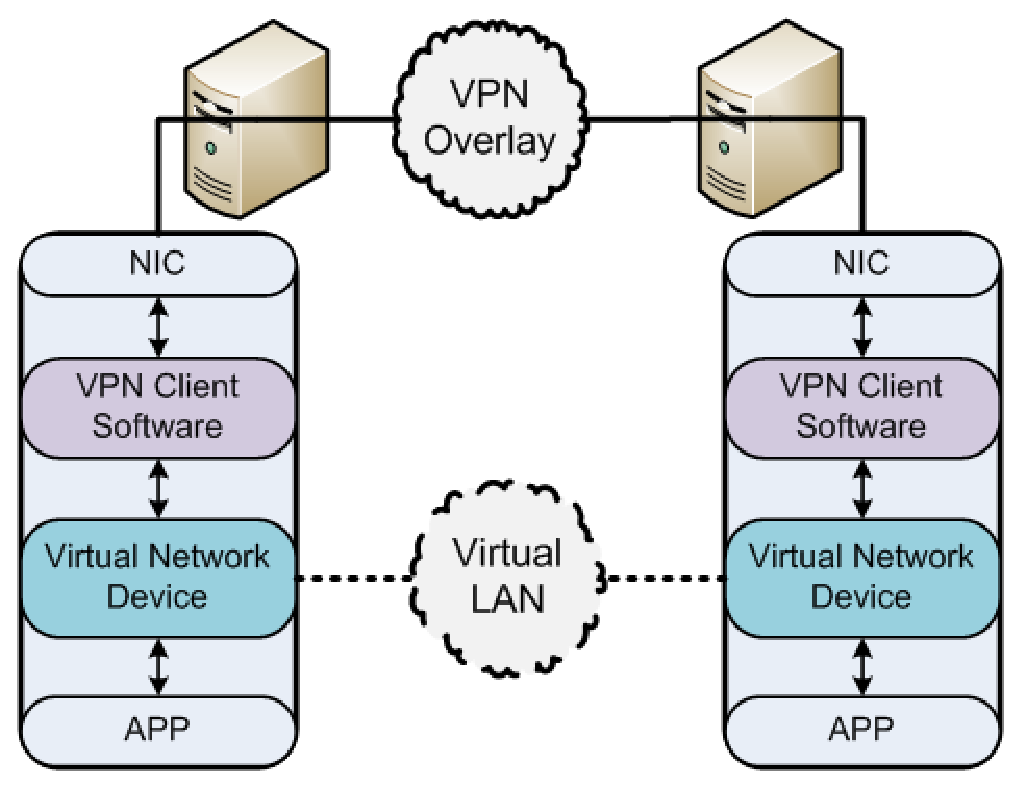
\epsfig{file=figs/vpn.png.eps, width=2in}
\caption{A typical VPN client.  A VN device makes application interaction with
the VPN transparent by integrating with the OS network stack.}
\label{fig:vpn}
\end{figure}

\subsection{Centralized VPN Systems}
OpenVPN is an open and well-documented platform for deploying centralized VPNs.
In this paper, it is used as the basis for understanding centralized VPNs as it
represents features common to most centralized VPNs.

In centralized VPN systems, clients forward all VPN related packets to the
server.  Client responsibilities are limited to configuring the VN device and
authenticating with the VPN server; whereas the servers are responsible for
authentication and routing between clients Likewise, broadcast and multicast
packets also must pass through the central server.

Centralized systems do not prohibit multiple servers, though each server must
be manually configured to interact with remote servers.  Clients randomly
select a server from a list of known servers, implementing a simple load
balance.  Once connected, the servers provide the client an IP address in the
VPN address space.  Thus two peers on different servers will have three hops
between each other, two from routing over the two servers and one for the
forwarding to the destination.

All inter-client communication flows through a central server.  By default, a
client encrypts a packet and sends it to the server.  Upon receiving the packet,
the server decrypts it, determines where to relay it, encrypts it, and then
sends the packet to its destination.  This model allows a server to eavesdrop on
communication.  While a second layer of encryption is possible through a shared
secret, it requires out-of-band communication and increases the computing
overhead on communication since the packet will now need to be encrypted and
authenicated twice at both the VPN source and destination sites.

\subsection{Centralized P2P VPN Systems}
Hamachi~\cite{hamachi} is the first well-known centralized VPN that used the
ambiguous moniker ``P2P VPN''.  In reality, these systems are better classified
as centralized VPN servers with P2P links.  Similar VPNs include
Wippien~\cite{wippien}, Gbridge~\cite{gbridge}, PVC~\cite{pvc}, and
P2PVPN\footnote{Due to the similarities between the name P2PVPN and focus of
this paper, ``P2PVPN'' refers to ~\cite{p2pvpn} and ``P2P VPN'' to to the use
of P2P in VPNs.}~\cite{p2pvpn}.  The P2P in these systems is limited to direct
connectivity between clients orchestrated through a central server: in Wippien
it is a chat server, while P2PVPN uses a BitTorrent tracker.  If NAT traversal
or firewalls prevent direct connectivity, the central server can act as a
relay.  Each approach uses their own security protocols with most using a
server to verify the authenticity and setup secure connections between clients.
In regards to the P2PVPN, long term goals involve the creation of an
unstructured, which would provide a method of decentralized organization.  A
disadvantage to the more robust approaches of Hamachi and GBridge is that they
do not allow network configuration, nor do they allow use without connecting
through their systems.

\subsection{Decentralized VPN Systems}
Some examples of systems that assist in distributing load in VPN systems are
tinc~\cite{tinc}, CloudVPN~\cite{cloudvpn}, ViNe~\cite{vine}, VNET~\cite{vnet},
and Violin~\cite{violin}.  These systems are not autonomic and require explicit
configuration of links between resources.  This means that, like OpenVPN, these
systems can suffer VPN outages when nodes go offline, thus administrators must
maintain the VPN connection table.  Unlike OpenVPN, these approaches typically
do not require all-to-all direct connectivity for all-to-all communication.
Users can either setup out-of-band NAT traversal or route through relays.

\subsection{Unstructured P2P VPN Systems}
Unlike centralized and decentralized systems, P2P environments require the
user to connect to the overlay, which then automatically configures links.
The simplest form of overlays are unstructured, where peers form random
connections with each other and use broadcast and stochastic techniques to find
information and other peers, though due to its unstructured nature, the system
cannot guarantee distance and routability between peers.  The only example of
an unstructured VPN is N2N~\cite{n2n}.  In N2N, peers first connect to a super
node and then, to find another peer, they broadcast discovery messages to the
entire overlay.  In the case that peers cannot form direct connection, peers
can route to each other over the N2N overlay.  In the realm of VPNs, all client
VPNs are also servers performing authentication though neither approach deals
with decentralized address allocation.  N2N does not address the challenges of
IP address allocation and management, relegating that to the user to handle.

\section{Structured P2P VPN Systems}
\label{structured_vns}
This section describes the basic construction of a Structured P2P VPN,
including background on structured overlays, address allocation and discovery,
security, and connectivity.

\subsection{Background}
An alternative to dealing with scalability concerns in unstructured systems,
structured overlays provide distributed look up services with guaranteed search
time with a lower bound of $O(\log N)$, in contrast to unstructured systems,
which rely on global knowledge/broadcasts, or stochastic techniques such as
random walks~\cite{unstructured_v_structured}.  Some examples of structured
systems are Pastry~\cite{pastry}, Chord~\cite{chord}, Symphony~\cite{symphony},
Kademlia~\cite{kademlia}, CAN~\cite{can}, and Brunet~\cite{brunet}.  In
general, structured systems make these guarantees by self-organizing into a
well-defined topology, such as a 2D ring or a hypercube, by randomly generated,
though uniformly distributed, node identifiers.  A key component of most
structured overlays is support for decentralized storage/retrieval of
information by mapping keys to specific node IDs in an overlay called a
distributed hash table (DHT).  At a minimum, the data is stored at the node ID
either smaller or larger to the data's node ID and for fault tolerance the data
can be stored at other nodes.  DHTs can be used by peers of systems to
coordinate allocation and discovery of resources, making them attractive for
self-configuration in decentralized collaborative environments.

\subsection{Organization}
In the context of VPNs, structured overlays can handle organization of the
network space, address allocation and discovery, decentrally through the use
of a DHT, such systems have been proposed in~\cite{pcgrid07,i3}.  Membership
in the VPN includes a matching membership in the structured overlay, thus all
VPN peers have a node ID.  To address the challenges of having multiple VPNs in
the same overlay, each VPN has its own namespace, reducing the likelihood of
overlap.  To enable scalable and decentralized address allocation and discovery,
peers store mappings of IP address to node ID into the DHT, typically of the
form $hash(namespace + IP) = node ID$.  Thus a peer attempting to allocate an
address will insert this key, value pair into the overlay.  The first peer to
do this will be the owner of the IP address allocation.  Therefore the DHT must
either support atomic writes into the DHT and prevent future writes or provide
creation times of key, value pairs during queries.

Mechanisms to self-configure the IP address and network parameters of the local
system can be provided by DHCP, manually configuring the IP address, or the VPN
hooking into OS APIs.  Address discovery is initiated when an outgoing packet
for a remote peer arrives at the VPN software.  At which point, the VPN will
query the DHT with the IP address to obtain the owner's node ID and forward the
packet to the destination.  Discussion on both these topics is further covered
in our previous work~\cite{sc09}.

\subsection{Privacy for the VPN}
Structured overlays are difficult to secure.  Malicious users can pollute the
DHT, send bogus messages, and even prevent the overlay from functioning.  When
using a structured overlay for a VPN, tamper-resistance and reliable routing
mechanisms are ideal, but they only reduce the ability of a malicious user to
affect the overlay, an expectation of a VPN is that no members are malicious
and malicious users have their access revoked.  As such a structured overlay
requires both the point-to-point (PtP), or communication between connected
peers, and end-to-end (EtE), or communication between peers across the
overlay, security.  Each component provides secrity uniquely from each other.
PtP security ensures that malicious third parties cannot insert material into
the system, while EtE ensures message security between the commuicating peers.
Enablng just PtP security would limit the security to the type of VPN security
found in other VPNs, all member must be trusted, whereas EtE enables message
security even from overlay members.

In our previous work~\cite{vpo}, we described mechanism that enable the
construction of a private overlay providing both EtE and PtP security.  In this
system, EtE and PtP communication has been abstracted into a common sender
layer; while the security component has been placed into a filter, enabling it
to be placed anywhere in the sending stack and thus securing either EtE or PtP
communication without additional complexity.  Existing security filter supports
DTLS~\cite{dtls}, as using DTLS does not require reliable communication across
the overlay or between peers.

\subsection{Connecting to the VPN}
As of 2010, the majority of the Internet is connected via Internet Protocol (IP)
version 4.  A limitation in this protocol is that there are only $2^{32}$
addresses (approximately 4 billion) available.  With the Earth's population of
over 8 billion and each individual potentially having multiple devices that
have Internet connectivity, the IPv4 limitation is becoming more and more
apparent.  To address this issue there have been two approaches:  1) the use of
network address translation (NAT) enabling many devices to share a single IP
address though limiting connection initiation, and 2) IPv6 which supports
$2^{128}$ addresses but comes with no guarantees of the demise of NATs or
firewalls that only allow outbound connections.

NATs and firewalls are impediments to P2P systems as they limit all-to-all
connectivity.  There has been much research to address these challenges, the
results come in the form of two types of NAT traversal: hole punching and
relaying.  When performing hole punching~\cite{ice}, peers exchanged IP and
port information through a third-party proxy and simultaneously attempt to
create "holes" in their NAT / firewall devices allowing direct TCP or UDP
communication with a peer behind another NAT / firewall.  This works by
confusing the NAT into believing that the peer behind it initiated the
connection.  TCP NAT hole punching, though, does not work on systems that use
stateful firewalls.  Relaying, on the other hand, always works as peers behind
NATs communicate through a third peer with whom they have have direct
connectivity, though with the side-effect of additional latency and the cost
incurred by the relay of supporting the bidirectional communication.

Creating and connecting to a private overlay can be difficult when there are
no dedicated resources with public addresses, even if the system has many
active members behind NATs and firewalls.  This is because peers behind NATs
and firewalls may be unable to handle incoming connections without the
assistance of a third-party.  The same work~\cite{vpo} describes how
abitrary public overlays can act as a middle ground to bootstrapping private
overlays, using mechanisms unique to these environments to bootstrap into the
private overlay.  Thus as mentioned in the introduction, peers can discover
each other using public overlays to connect to a private overlay.  The key
challenge to using public overlays is that they must allow peers to send
abitrary data to each other via the overlay, otherwise two peers behind NATs
will be unable to coordinate NAT traversal with each ohter.  Of course, this
mechanism does not preclude the creation of a private overlay without the
use of a public bootstrapping mechanism.

In practical implementation, peers first join a public structured overlay using
the public overlay's DHT to find other peers.  The private overlay node can then
either attempt to connect directly with other private overlay nodes using TCP or
UDP or use the public overlay as another transport mechanism.  We have termed
this approach to creating private overlays, virtual private overlays.  In all
cases, the communication is secured via the EtE and PtP security filters.  This
approach enables the construction of an overlay consisting entirely of peers
behind NATs and firewalls, who would otherwise be unable to form their own
overlay.

\subsection{Managing and Configuring the VPN}
\label{groups}
A Group based Web 2.0 environment enables low overhead configuration of
collaborative environments.  The roles in a group environment can be divided
into administrators and users.  Users have the ability to join and create
groups; whereas administrators define network parameters, accept or deny join
requests, remove users, and promote other users to administrators.  By applying
this to a VPN, the group environment provides a wrapper around a public key
infrastructure (PKI), where the administrators of the group act as the
certificate authority (CA) and the members have the ability to obtain signed
certificates.  Elaborating further, when a user joins a group, the
administrator can enable automatic signing of certificates or require prior
review; and when peers have overstayed their welcome, an administrator can
revoke their certificate by removing them from the group.  As described
in~\cite{vpo}, revocation can be stored as a CRL on the group site or
distributed through broadcast and DHT on the overlay.  Though for these forms
of systems a user revocation list (URL) as opposed to a CRL simplifies
revocation in the case where a malicious user has automatically signed large
amounts of certificates.

In the case of the GroupVPN, administrators of a group configure the VPN
address range, namespace, and security.  Options are also available to specify
the reuse of an existing public overlay or a list of user managed nodes.  When
a user has been accepted into the group, they are able to download VPN
configuration data, which can be seamlessly added to the VPN by running the
VPN configuration process.  In addition to IP address range, namespace, and
security options, the configuration data also contains the group website's
address and a shared secret.  The shared secret uniquely identifies the user,
so that the website can automatically sign the certificate or enqueue it so the
administrator can manually sign it.  When making a certificate request, the
user sends over HTTPS a public key and their shared secret, the website creates
and signs a certificate request based upon the public key and the user's
relevant information ensuring that users cannot trick the website into signing
malicious data.  Upon receiving the signed certificate, peers are able to join
the private overlay and VPN enabling secure communication amongst the VPN peers.

There are many ways of implementing and hosting the web site.  For example, Google
offers free hosting of Python web applications through Google Apps, but this
requires that the user owns a domain.  Alternatively, the user could host the
group site on a public VN, peers interacting with the GroupVPN would need to
connect with the public VN in order to create an account, get the configuration
data, and to sign their certificate at which point they could disconnect from
it.  This does not preclude the use of other social mediums nor a central site
dedicated to the formation of many GroupVPNs.  As many GroupVPNs can share a
single site, so long as the group members trust the site to host the CA private
key.

\section{Efficiently Dealing with NATs and Firewalls}
\label{relays}
Centralized and decentralized VPNs do not suffer from connectivity limitations
due to NATs and firewalls as all traffic passes through the central server or
managed links.  In the centralized P2P approaches, peers that cannot form direct
links can potentially route through a dedicated relay system, but if not, the
peers will be unable to communicate.  Whereas in decentralized approaches,
including P2P systems, peers can communicate through the overlay when traversal
fails.  Though as the overlay grows in size, especially in structured overlays,
so does the hop count between peers, increasing latency and reducing bandwidth,
greatly reducing the value of routing through an overlay.

\subsection{An Autnomic Relay Infrastructure}
\begin{figure}[ht]
\centering
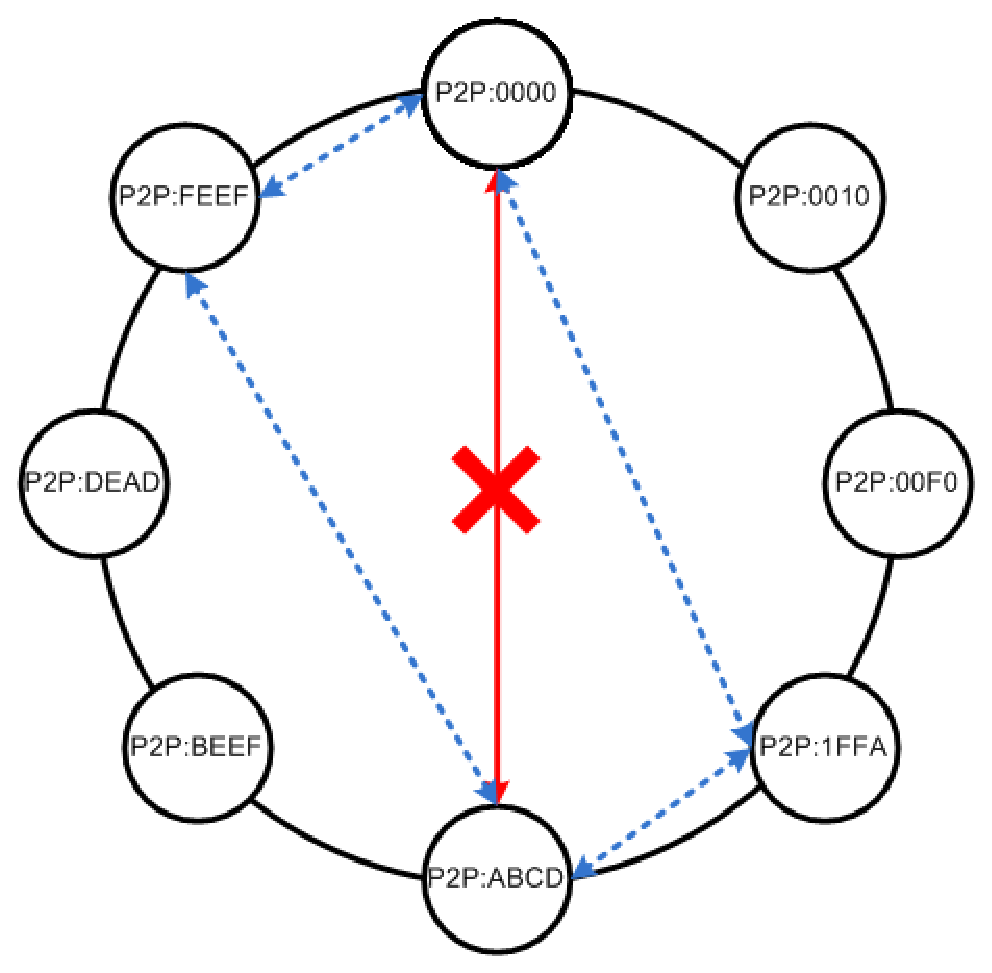
\epsfig{file=figs/relay.png.eps, width=2.75in}
\caption{Creating relays when direct connectivity is not possible.  Two members,
0000 and ABCD, are unable to form direct connectivity, thus they exchange
neighbor information through the overlay and connect to one of each other's
neighbors, creating an overlap.  The overlap then becomes a relay path
(represented by dashed lines) for two-hop communication.}
\label{fig:relay}
\end{figure}

P2P systems can address this connectivity issue through a distributed, autonomic
relaying system, whereby peers form overlapping connections with each others
peers, creating two-hop links.  When two nodes discover each other via the
overlay and attempt to become connected but fail during NAT and firewall
traversal, they exchange peer lists through the overlay.  Upon receiving this
list, the two peers identify the overlap in the neighbor sets to form a two-hop
connection.  When peers are not located near each other in the overlay, most
likely they will have no overlap.  This can be addressed by having peers
connect to each other's neighbor set proactively creating overlap, as
represented in Figure~\ref{fig:relay}.

With the set of neighbors, the peers can include additional data such as
latency and connection lifetime to each of the the neighbors.  When creating
overlap or overlap changes, peers review these metrics to decide which subset
of the overlap to use as a proxy leaving the remaining peers as reserves.

\subsection{Usefulness of Relays}
To determine the value in two-hop overlays as opposed to using the overlay in
restrictive NAT and firewall scenarios, this experiment uses a network modeler
that reuses the code base of the GroupVPN to faithfully implement routing in an
overlay as well as latency between peers.  Pair-wise latency in this experiment
is set using the MIT distribution of the King Data Set~\cite{king_data},
consisting of all-to-all latency for 1,740 distributed Internet peers.  The
modeler randomly assigns each peer in the modeler a matching physical location
based upon the data set, thus for simulations of over 1,740, peers may be
co-located.  The modeler measured average overlay, 2-hop, and 1-hop latency
between peers.  Overlay latency represents the time to route a packet via the
overlay.  2-hop latency is based upon the low-latency formed 2-hop connections,
where peers route over the overlap with the lowest latency.  1-hop latency is
based upon peers forming a direct connection with each other.  Only peers that
are not directly connected (i.e., have two hops or more and are not located in
the same physical location) are analyzed, as these situations would only benefit
under triangular inequalities, which are not a consideration in this work.

\begin{figure}[ht]
\centering
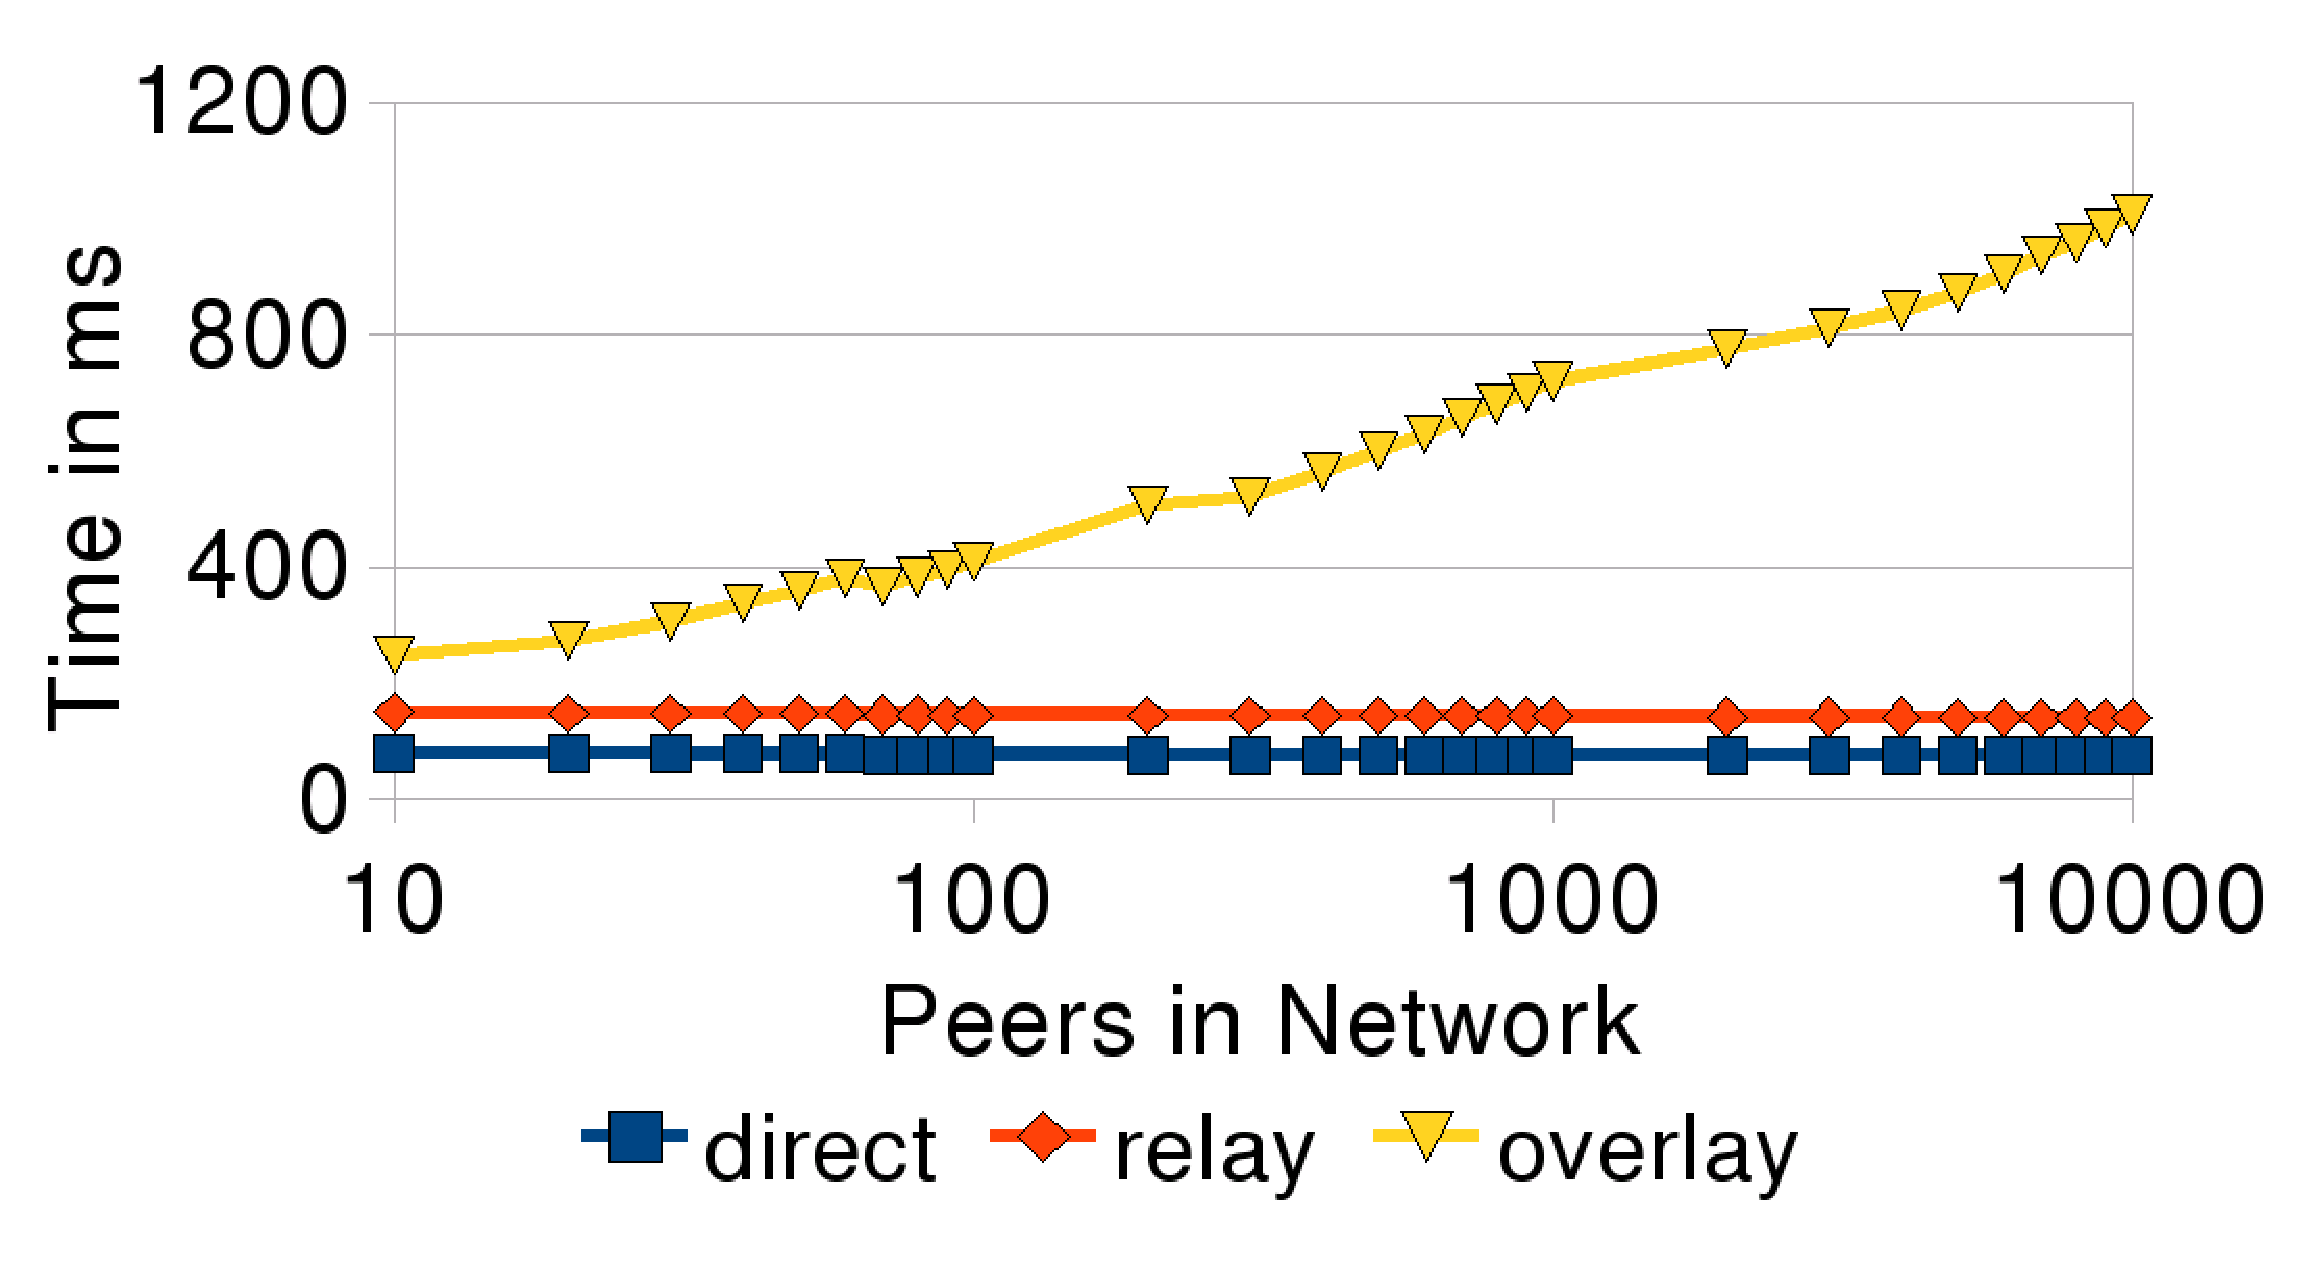
\epsfig{file=figs/relay_motivation.png.eps, width=2.75in}
\caption{A comparison of the average all-to-all overlay routing, two-hop relay, and
direct connection latency in a ring based structured overlay.}
\label{fig:simulated_relays}
\end{figure}

Results are presented in Figure~\ref{fig:simulated_relays}.  Immediately the
two-hop routing shows improvement.  While the overlay grows logarithmically,
the results for direct and relay remain nearly identical.  Clearly when
timing, which can affect bandwidth, is critical, direct paths are most desired,
though when they are not available, this experiment clearly shows that two-hop
paths, or relays, are significantly better than routing the packet through an
overlay.

In addition, the relays functionality were verified in GroupVPN using a real
system consisting of PlanetLab as the public overlay and the Archer as the VPN
environment.  PlanetLab~\cite{planetlab} provides a set of over 500 distributed
computing nodes all with public IP addresses.  Archer provides grid computing
to computer architecture researchers and consists of over 500 nodes located at
various academic sites.  To ensure that peers under study formed two-hop
connections, a firewall was instantiated preventing direct communication between
the two.  In tests, it was revealed that the overlay was always able to
self-configure a relay; the bandwidth and latency averages and deviations were
2245 Kbit/s $\pm$ 1080 and 58.1 ms $\pm$ 35.5, respectively.

\section{Efficient Broadcast and Multicast}
\label{efficient_xcast}
Within the past few years, self-configuring protocols like zeroconf and Bonjour
have enabled the use of complex applications transparently through
self-configuring, these include music sharing applications, like iTunes, chat
programs, like Pidgin, and even web sites and data shares.  The underlying
enabling technology is multicast DNS and service discovery.  Multicast has
also been used in other applications to enable efficient streaming of media,
such as music and videos.  These types of applications and enabling are ideal
for small and medium groups.

Many VPN technologies either do not support multicast and broadcast or route
the packets to all peers or through a central server, which may be reasonable
for relatively small groups and for discovery, but they do not scale well for
media streaming or lrage groups.  In the original set of structured P2P virtual
networks, broadcast and multicast used the DHT to keep a list of all the active
peers in the VPN.  When a peer wanted to send out a broadcast or multicast
packet, it would query this list and then send out unicast packets to each peer
either directly or via the overlay.  Furthermore, as more peers join the system,
so does the count of key, value pairs in the DHT.  If the peer wishes to send
out many multicast or broadcast messages after another, it would either need to
query the DHT every time or maintain a cache.  In the case of a cache, new
peers joining the overlay would need to notify the entire VPN when they joined
so that they could be added to caches.  The simplistic approach of querying
each time does not scale well, while the other approach involving caches can be
quite complciated to implement.

\subsection{Overlay Broadcast}
With the use of virtual private overlays, broadcast and multicast can be
implemented stateless as they can be routed using overlay broadcast.  An
example of a scalable ring-based structured P2P overlay broadcast algorithm
was presented in~\cite{vpo} to broadcast certificate revocation within a private
overlay.  The algorithm is called bounded-broadcast, because it is capable of
broadcasting to a subset of the ring or the entire overlay.  Bounded broadcast
uses the following recursive algorithm:  Begin with node $x$ triggering a
broadcast message over the region $[x, y]$.  $x$ has $F$ connections to nodes
in the range $[x, y]$.  Denoting the $i^{th}$ such neighbor as $b_i$, the node
$x$ sends a bounded broadcast over a sub-range, $[b_i, b_{i+1})$, to $b_i$,
except the final neighbor.  Differently stated, $b_i$ is in charge of
bounded-broadcasting in the sub-range $[b_i, b_{i+1})$. If there is no
connection to a node in the sub-range, the recursion has ended.  The final
neighbor, ($b_F$), is responsible for continuing the bounded broadcast from
$[b_F, y]$.  When a node receives a message to a range that contains its own
address the message is delivered to that node and then routed to others in that
range.  Figure \ref{fig:tree} shows how this bounded broadcast forms a local
tree recursively.   The time and bandwidth for a bounded broadcast is
$O(\log^2 N)$ and $N * packet size$ as shown in~\cite{small_world}.

To perform a broadcast on the entire overlay, a peer performs the
bounded-broadcast starting from its node ID with the end address being the node
ID immediately preceding its own in the address space.  Though in VPN
situations, many peers may already have connections to most if not all of their
VPN peers, thus the broadcast algorithm has been modified to route to only
connections created for structured overlay purposes and not explicitly only for
VPN purposes.  Otherwise in many cases, this algorithm will degenerate into one
similar to the unicast approach.

\begin{figure}[h]
\centering
\includegraphics[width=2.25in]{figs/tree.eps}
\caption{Bounded Broadcast in range $[x, y]$}
\label{fig:tree}
\end{figure}

Another consideration, left unexplored, is whether or not to create separate
overlays for each multicast group.  In IP multicast, peers register group
membership using IGMP (Internet Group Management Protocol), thus a VPN can be
configured to parse these packets and join a unique private overlay for that
multicast group.  In general, the cost of joining an additional overlay is
minimal, though, when used for zeroconf like applications, most peers will join
the group and more importantly the traffic is minimal anyway.  

\subsection{IP Broadcast Evaluation}
The broadcast validation was done using the same modeler used in the relay
evaluation.  This evaluation compares broadcasting to a simple unicast
mechanism that assumes the peer has already queried the DHT.  Both models are
evaluated in a private overlay varyin from 10 members up to 10,000.  It is
important to note that the network modeler does not consider host overheads
including bandwidth limitations nor simulataneous packet sending, thus the
results are from an ideal system.  The modeler measures network bandwidth,
sending peer bandwidth, and the time to complete the broadcast.  The results
are presented in Figures \ref{fig:broadcast_time} and \ref{fig:broadcast_hops}.

\begin{figure}[h]
\centering
\includegraphics[width=2.5in]{figs/broadcast_time.eps}
\caption{Time to complete an IP Broadcast}
\label{fig:broadcast_time}
\end{figure}

\begin{figure}[h]
\centering
\includegraphics[width=2.5in]{figs/broadcast_hops.eps}
\caption{Peers the broadcast packet traversed}
\label{fig:broadcast_hops}
\end{figure}

The timing results (Figure~\ref{fig:broadcast_time} indicate that the overlay
broadcast never takes longer than the unicast broadcast.  Another interesting
result was that the broadcast mechanism seems to avoid some of the longer paths.
This result is most likely related to the fewer packets sent across the network.
In Figure~\ref{fig:broadcast_hops}, the unicast broadcast can easily consists of
$N$ outgoing messages representing somewhere around $\log(N) * N$ hops, whereas
the overlay broadcast mechanism will always be $N$ hops.  In smaller networks
this does not have a significant effect in terms of network utilization, but
from the perspective of the broadcast originator, having to send $\log(N)$
messages as compared to $N$, can save significant bandwidth.  So beyond being
stateless, the approach is not only more efficient in terms of bandwidth but all
peers receive the message in a reasonable amount of time.

\section{Evaluation of VPN Models}
\label{evaluation}
This experiments explores bandwidth and latency in a distributed VPN system to
motivate the usage of P2P links in a VPN.  The VPNs used are include our
GroupVPN, OpenVPN, and Hamachi.  OpenVPN represents a typical
centralized VPN, while Hamachi represents a well-tuned P2P-link VPN.  The
evaluation was performed on Amazon EC2 using small instance sized
Ubuntu i386 instances to create various sized networks ranging from 1 to 32.
OpenVPN uses an additional node as the central server and Hamachi has an upper
bound of 16 due to limitations in the Linux version at the time of this
evaluation.  To perform bandwidth tests, the instances are booted and query an
NFS for the list virtual IP addresses, peers are ordered such that half the
peers are act as clients and the other half the peers creating a 1 to 1 mapping
between all sets.  Latency and bandwidth tests are performed using netperf's
request-reply and streaming tests respectively.  Prior to the start of the
tests, peers have no knowledge of each other, except the virtual IP addresses,
thus connection startup costs are included in the test.  Test are run for 10
minutes diluting the connection initiation overhead but represent an example of
real usage.  Results from the clients are polled at all locations and averaged
together, though the OpenVPN server is measured separately.  GroupVPN and OpenVPN
use authenticated 128-bit AES, while Hamachi does not allow configuration of
the security parameters and uses the default Hamachi settings, 256-bit AES.

\begin{figure}[ht]
\centering
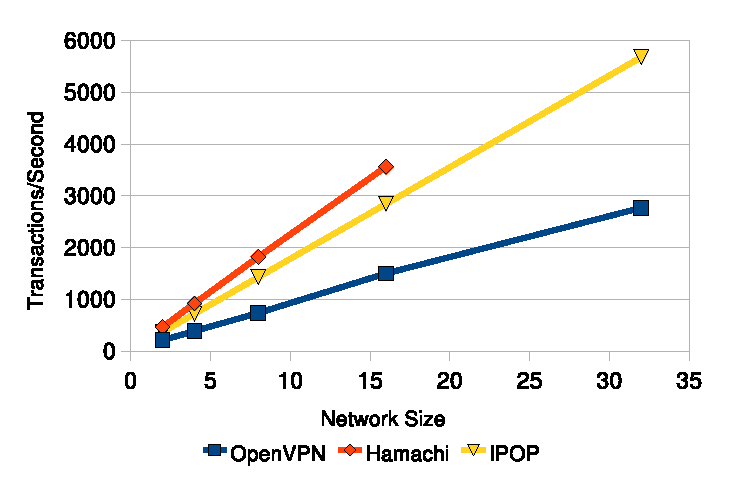
\epsfig{file=figs/latency.eps, width=2.5in}
\caption{System transaction rate for various VPN approaches.}
\label{fig:latency}
\end{figure}

\begin{figure}[ht]
\centering
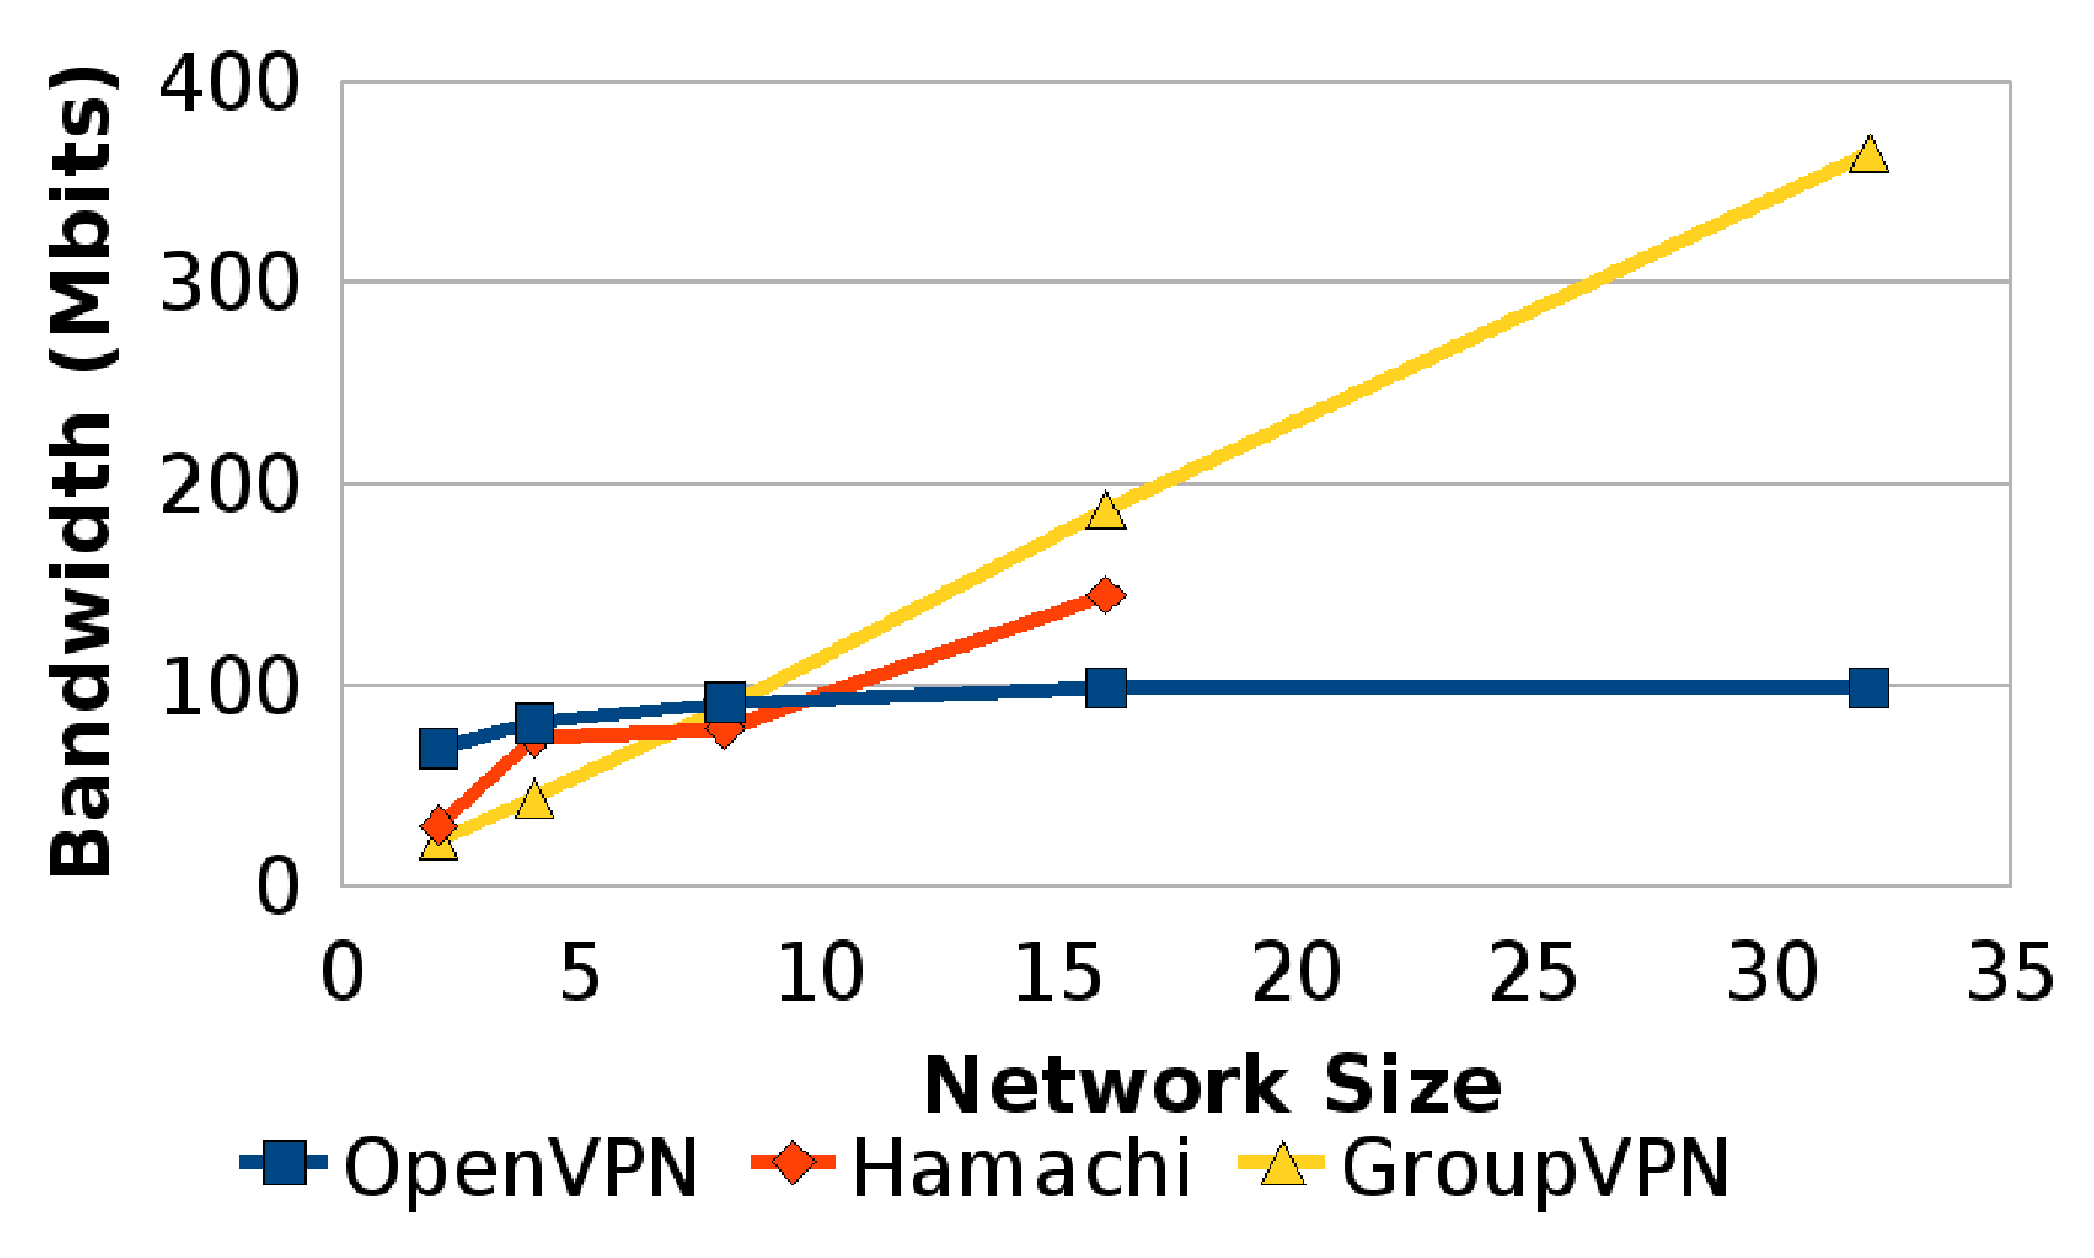
\epsfig{file=figs/bandwidth.eps, width=2.5in}
\caption{System bandwidth for various VPN approaches.}
\label{fig:bandwidth}
\end{figure}

Figures \ref{fig:latency} and \ref{fig:bandwidth} present the results for latency
and bandwidth respectively.  Latency is measured in transactions of successful
request/reply messages.  In the latency test, it is obvious that having the
central server increases the delay between the client and server and the results
degrade more quickly as additional peers are added to the system.  In small
systems, OpenVPN shines probably due to optimized software, though as the system
grows, the system bandwidth does not.  By the time 8 peers have entered into
the system, both decentralized approaches perform better than the OpenVPN
solution.  To summarize, decentralized VPN approaches provide better
scalability, which can be immediately noticed by low latency times and, as the
system grows, available bandwidth.

\section{Conclusions}
\label{conclusions}
This paper describes a novel approach to VPNs utilitizing structured overlays
to deal with organization, public overlays for connectivity, private overlays
for security, and collaborative web environments for configuration and
management.  The paper furthers previous work done by virtual private overlays
to enhance key VPN features, relays and IP broadcast and multicast.  

Without GroupVPN projects like Archer~\cite{archer}, would be impractical.
Archer consists of over 500 resources from 5 different universities,
including University of Florida, Florida State University, Northeastern
University, University of Minnesota, and University of Texas.  In the past
year, since Archer came online, over 100 unique users have contributed and taken
advantage of the voluntary computing cycles.  A new user to the system begins by
creating an account at \url{Grid-Appliance.org} and requesting membership in the
Archer GroupVPN group.  Once access has been granted, users can obtain
configuration data that enables them to seamlessly add resources to the grid by
handing the configuration file to the Grid Appliance initialization scripts.
This method allows independent submission sites, unlike most grid systems that
have a shared submission site, which require dedicated administrators.  Most
users connect to the system using a pre-configured virtual machine appliance,
so that they do not need to be experts in grid systems to take advantage of
Archer.  GroupVPN allows users to connect to the system and dynmaically add
resources.  In the case of decentralized VPNs, this would be difficult as the
user would need to create a manual link to the rest of the system for each new
resource.  N2N may work, but the network size of Archer is larger than the
recommendations made by N2N and would still require the setup of address
allocation facilities.  In general, all existing approaches would fail besides
those with centralized components, because, at the time of this writing, all of
Archer's resources are behind NATs.  While centralized could be used, they
would require additional dedicated resources and management and limit access if
the central component went offline.

In addition to Archer, the components in GroupVPN have been used to construct
a VPN that uses online social networking identities to establish trust, called
SocialVPN~\cite{cops08}.  The GroupVPN has been used to construct Grid Appliance
that enables the creation of distributed, decentralized, dynamic computing
grids, which form the basis for Archer.  Recently, a grid at La Jolla Institute
for Allergy and Immunology went live using GroupVPN and Grid Appliance without
receiving any technical support from us.  Researchers at Clemson University and
Purdue have opted for this approach over centralized VPNs as the basis of their
future distributed compute clusters and have actively tested networks of over
700 nodes.
\bibliographystyle{IEEEtran}
\small{
\bibliography{GroupVPN}
\suppressfloats
}

\end{document}
